\documentclass[17pt]{beamer}
\usetheme{Warsaw}
\usepackage[utf8]{inputenc}
\usepackage{amsmath}
\usepackage{amsfonts}
\usepackage{amssymb}
\usepackage{graphicx}
\author{B.TEJA,P.PRANEETH,PRANJAL}
\title{FINDING THE EQUATION OF CIRCLE}

\begin{document}

\begin{frame}
\titlepage
\end{frame}
\begin{frame}[t]{Question}
If the line 2x+3y+1=0 and 3x-y-4=0 lie along the diameters of a circle of circumference $10\pi$
 then the equation of the circle is ?
\end{frame}
\begin{frame}[t]{Solution}
given equations are

\hspace{5cm}
$\begin{bmatrix}
2&3
\end{bmatrix}x=-1$

\hspace{5cm}
$\begin{bmatrix}
3&-1
\end{bmatrix}x=4$

and circumference of circle is $10\pi$

by solving 
we will get the intersection point as 
$\begin{bmatrix}
1\\
-1
\end{bmatrix}$
\end{frame}
\begin{frame}
We know that the circumference of the circle is $2\pi$r
As the given circumference is $10\pi$


\hspace{3cm}
$2\pi
r$
=
$10
\pi$


therefore 

radius of given circle is (r=5)

\end{frame}
\begin{frame}
we know that the equation of circle with centre 
\[C=\begin{bmatrix}
1\\
-1
\end{bmatrix}\]

\hspace{3cm}
 \[ \Vert(X-C)\Vert^2
 =r^2\]
 \[(X-C)^T (X-C)
 =r^2\]
 \[X^T X
 -2C^T X
 =
 r^2
 -C^T C\]
  \end{frame}
 \begin{frame}
 by substituting the centre C
 equation of the circle is 

 $X^T X$-
   $\begin{bmatrix}
1&-1
\end{bmatrix}X$
=$r^2$ - $\begin{bmatrix}
1&-1
\end{bmatrix}$$\begin{bmatrix}
1\\
-1
\end{bmatrix}$

therefore
\[x^2
+
y^2
-2x
+2y
-23
=0\]

is the required circle equation
\end{frame}
\begin{frame}[t]{Extra}
x=$rcos(\Theta)$ +h
y=$sin(\Theta)$ +k

by differentiating
slope of circle at $\Theta$ is

m = -$cot\Theta$

as we know the values of $\Theta$ by the given line equations
we will get the slopes of tangents at 4 intersection points
 now we will find tangent equations from slope and point
 
\end{frame}
\begin{frame}
we will get the 4 intersection points of tangents 

now we can find the area of one triangle by $(base *height)$$\div2$

now the area of quadrilateral is 2*area of triangle
\end{frame}
 \begin{frame}
 \begin{figure}[b]
\centering
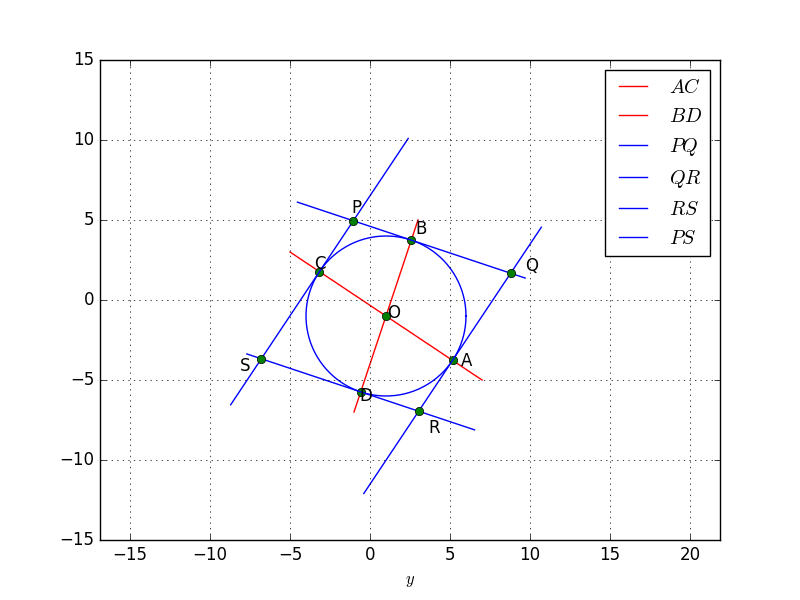
\includegraphics[width=1\textwidth]{wowd.png}
\caption{area of triangle}
\end{figure}
\end{frame}
\end{document}
